% !TeX program = xelatex
\documentclass[a4paper,utf8]{ctexart}
\usepackage{report}

\def\mytitle{实验报告标题}
\def\mysubtitle{实验报告副标题}
\def\name{姓名}
\def\sno{学号}
\def\institution{学院}
\def\email{xxxx@xxx.edu.cn}

\title{
    \vspace{-2cm}
    \hrule  height 2pt \relax
    \vspace{.5cm}
    {\color{DarkRed}
    \heiti{\huge \mytitle}\\
    \mysubtitle
    }
    \vspace{.5cm}
    \hrule height 1pt \relax
    }

\author{\name\\
    \sno\\
    \institution\\
    \color{DarkRed}
    \href{mailto:\email}{\fontfamily{qcr}\selectfont\email}
    }

\date{\today}


\begin{document}

\maketitle

\section{一级标题}
\subsection{二级标题}\label{sec:sec1}

\section{文本}
\subsection{列表}
\begin{itemize}
    \item 无序列表
    \item 无序列表
\end{itemize}

\begin{enumerate}
    \item 有序列表
    \item 有序列表
\end{enumerate}

\subsection{符号}
使用 \verb|fontawesome| 宏包, 如 \faGithub, \faLink. \href{http://mirrors.ibiblio.org/CTAN/fonts/fontawesome/doc/fontawesome.pdf}{宏包文档}.

\subsection{链接}
\href{https://ysyszheng.github.io/}{网址}, 图~\ref{fig:example}, 表~\ref{tab:short}, ~\ref{tab:long}, 章节~\ref{sec:sec1}.

\section{代码}
行内代码 \verb|import numpy as npy| .
行间代码:
\begin{lstlisting}[language=C]
struct map {
    unsigned m_size;
    char *m_addr;
    struct map *next, *prior;
};
struct map *coremap;
\end{lstlisting}

% \lstinputlisting[language=C]{./code/name.c}

\section{图片}
\begin{figure}[H]
    \centering
    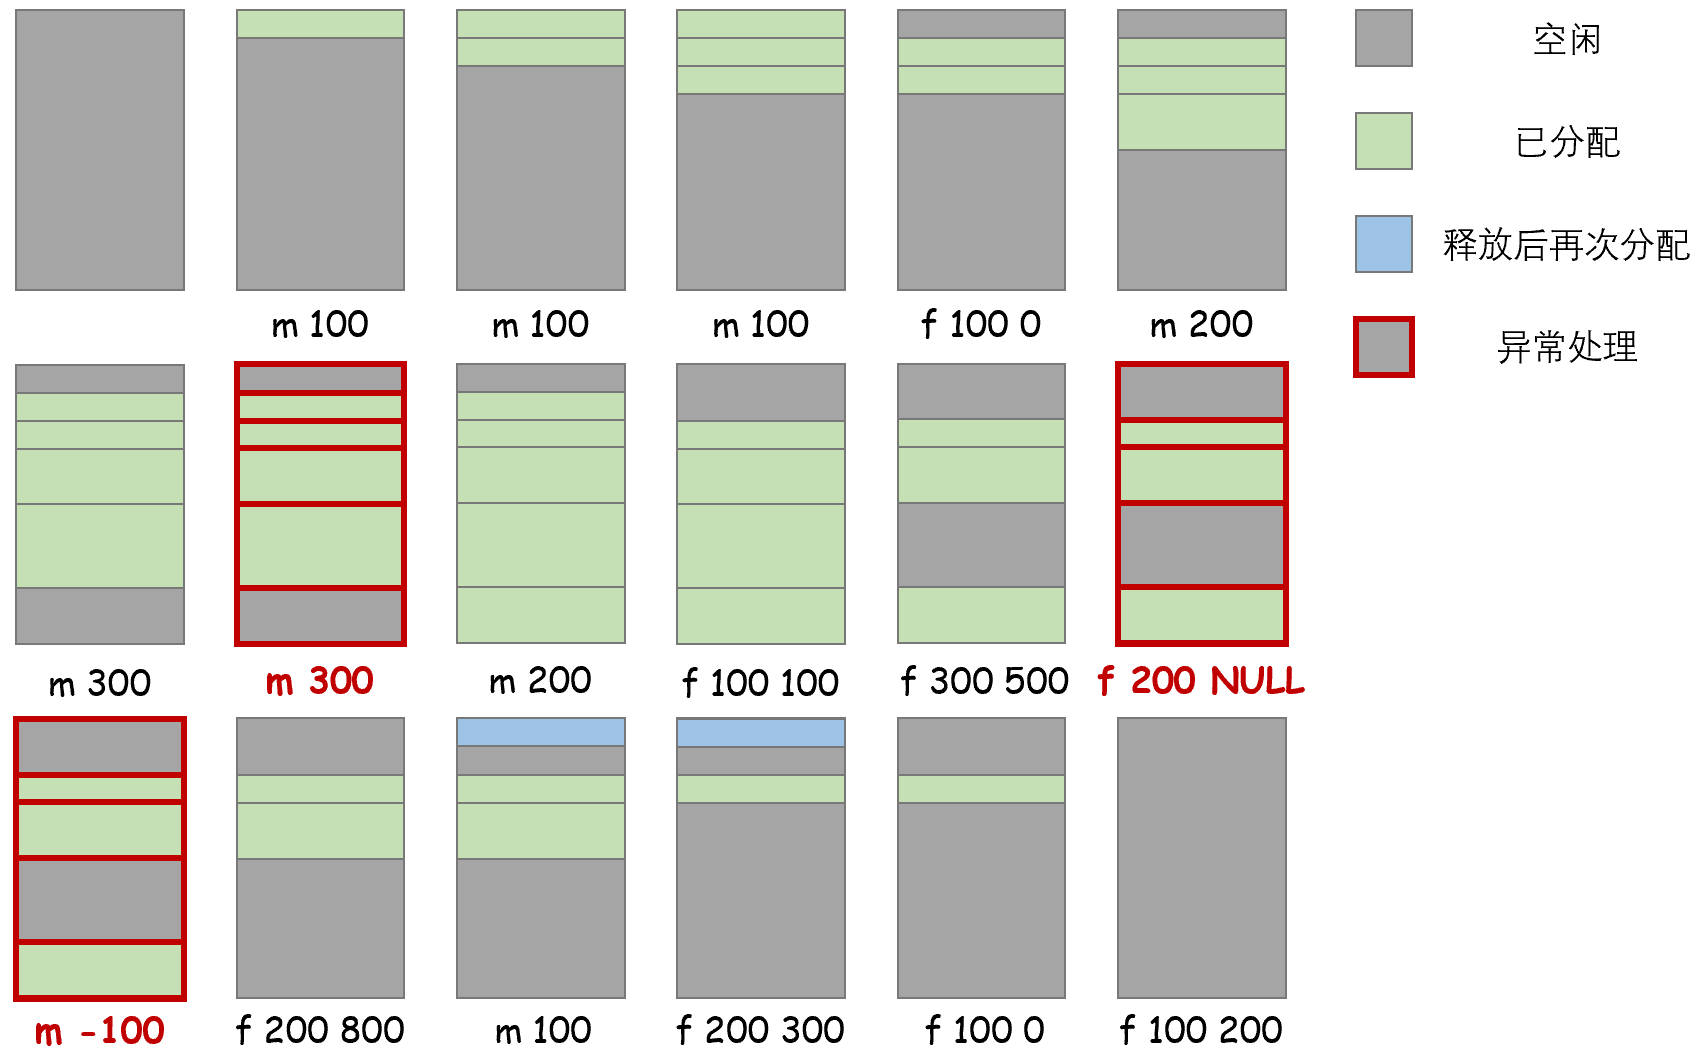
\includegraphics[width=\textwidth]{./img/example.jpg}
    \caption{测试用例示意图}
    \label{fig:example}
\end{figure}

\section{表格}

\begin{table}[ht]
    \centering
    \caption{三线表样例}
    \begin{tabular}[t]{lcc}
    \toprule
    &A&B\\
    \midrule
    aaa&1&2\\
    bbb&--&3\\
    ccc&4&5\\
    \bottomrule
    \end{tabular}
    \label{tab:short}
\end{table}

\begin{sidewaystable}[htbp]
    \centering
    \caption{长表格样例}
    \begin{tabular}{lccccccccc}
    \toprule
    \multirow{2}*{} & \multicolumn{3}{c}{Owner} & \multicolumn{3}{c}{Renter}&\multicolumn{3}{c}{All}\\
    \cmidrule(lr){2-4} \cmidrule(lr){5-7}\cmidrule(lr){8-10}
    &(1)&(2)&(3)&(4)&(5)&(6)&(7)&(8)&(9)\\
    \midrule
    \multirow[t]{2}*{Log of housing prices}&.082$^{***}$&.069$^{***}$&.067$^{***}$
    &.063&.121&.104
    &.833$^{***}$&.065$^{***}$&.064$^{***}$\\
    &(.006)&(.011)&(.011)
    &(.064)&(.084)&(.088)
    &(006)&(.010)&(.010)\\
    \multirow[t]{2}*{Log of household income}&.131$^{***}$&.086$^{***}$&.086$^{***}$
    &.010&-.002&-.002
    &.132$^{***}$&.086$^{***}$&.086$^{***}$\\
    &(.005)&(.009)&(.009)
    &(.034)&(.041)&(.042)
    &(.005)&(.009)&(.009)\\
    \multirow[t]{2}*{Log of house size}& &.040$^{**}$&.038$^{*}$
    & &.076&.071
    & & .035$^{*}$&.034$^{*}$\\
    &&(.020)&(.020)
    &&(.109)&(.111)
    & & (.019)&(.019)\\
    \multirow[t]{2}*{Log of savings}& & .008$^{***}$&.008$^{***}$
    & & -.005 & .071
    & & .008$^{***}$&.008$^{***}$\\
    & & (.002)&(.002)
    & &(.013)&(.014)
    & &(.002)&(.002)\\
    \multirow[t]{2}*{Log of mortgage}& &.013$^{***}$ &.013$^{***}$
    & & -.002 & -.004
    & &.012$^{***}$&.012$^{**}$\\
    & & (.005)&(.005)
    & &(.027)&(.029)
    & &(.005)&(.005)\\
    \multirow[t]{2}*{Log of debts}& & .019$^{***}$&.019$^{***}$
    & &.002 &.00005
    & &.019$^{***}$&.018$^{***}$\\
    & & (.002) & (.002)
    & &(.011)&(.012)
    & &(.002)&(.002)\\
    \multirow[t]{2}*{Family size}& & .106$^{***}$&.106$^{***}$
    & & .169&.178$^{*}$
    & &.109$^{***}$&.109$^{***}$\\
    & &(.010)&(.010)
    & &(.105)&(.106)
    & &(.010)&(.010)\\
    \multirow[t]{2}*{Log of provincial GDP}& & &.198
    & & &.665
    & & &.194\\
    & & &(.123)
    & & &(.832)
    & & &(.113)\\
    \multirow[t]{2}*{Unemployment rate}& & &.016
    & & &.0651
    & & &.022\\
    & & &(.034)
    & & &(.160)
    & & &(.032)\\
    \midrule
    Household FE&\Checkmark&\Checkmark&\Checkmark&\Checkmark&\Checkmark&\Checkmark&\Checkmark&\Checkmark&\Checkmark\\
    Time FE&\Checkmark&\Checkmark&\Checkmark&\Checkmark&\Checkmark&\Checkmark&\Checkmark&\Checkmark&\Checkmark\\
    Control Var.&&\Checkmark&\Checkmark&&\Checkmark&\Checkmark&&\Checkmark&\Checkmark\\
    Provincial Macro Var.&&&\Checkmark&&&\Checkmark&&&\Checkmark\\
    Obs&24,100&10,519&10,519&509&332&332&24,614&10,854&10,854\\
    R-Square&0.3216&0.3415&0.3235&0.2167&0.2719&0.1674&0.3219&0.3397&0.3246\\
    \bottomrule
    $^{***} p<.01, ^{**} p<.05, ^{*} p<.1$
    \end{tabular}
    \label{tab:long}
\end{sidewaystable}

\section{数学公式}
\begin{equation}
    a^2+b^2=c^2
\end{equation}

\appendix

\section{附录名称}

\end{document}
